
\chapter{Implementation}

In this chapter, I will explain how I implemented my solutions.

\section{Application}

First of all, I implemented the application for the tests. I choose to implement this application in python and it
is hosted on the computer named Dedian (cf figure \ref{fig:network}). As it was explain in the chapter
\ref{chap:choice}, this application has three state: Ping, Pong and Admin.

Considering I have to implement the defense of this application, I have to delimit the sensitive space. It is
obvious for this application, the sensitive state is the admin state. So I have to send many event when the user
try to access to the admin interface. In this way I could know if somebody try without success to access to the
admin interface, this person is doubtless an attacker.

To raise event, I send message to a particular Logstask instance which is on SELKS. This message contain the time
and the state of the application. I will explain after, how the Logstash instance work.

\begin{table}[h]
  \centering
  \begin{tabularx}{1.0\linewidth}{|X|X|}
    \hline
    Hosted&Debian\\
    \hline
    Language & Python \\
    \hline
    States & Ping, Pong, Admin \\
    \hline
    Sensitive state & Admin \\
    \hline
    Port open & 9124, 9000\\
    \hline
    Outdoor communication & Selks to port 5000 \\
    \hline
    Port 9124 accept communication from & Everybody \\
    \hline
    Port 9000 accept communication from & Metasploitable only\\
    \hline
  \end{tabularx}
  \caption{Features of the application}
  \label{tab:carac}
\end{table}


\section{Probe}

\subsection{Network probe}

I already explain that I use SELKS as IDS, but I had to configure it to adapt it to my application. So I had rules
on the Suricata ruleset. To add rules, I use the scirius interface which permit to administrate suricata's ruleset.
I added the next rules:

\begin{lstlisting}[language=suricata]
  alert tcp any any -> any 9124 (msg:"Action goping"; \
  content:"goping"; sid:501; rev:5000;)

  alert tcp any any -> any 9124 (msg:"Action gopong"; \
  content:"gopong"; sid:502; rev:5001;)

  alert tcp any any -> any 9000 (msg:"Connexion vers l interface admin"; \
  flow:established,to_server sid:504; rev:5002;)
\end{lstlisting}




\subsection{Application probe}

As it was explain before, to have the status of the application, it sends to Logstash its status. Then Logstash
filter these messages and write them on the Elasticsearch data base.

On the SELKS computer, there is a Logstash implemented with a filter adapted for Suricata but not for our
application. So I write a filter to Logstash adapted for this application, and I run a new instance of Logstash
with this configuration on SELKS. By this way, both instance of Logstash do their job without interaction.

The filter implemented, convert plain text message send by my application as json event readable by Elasticsearch.
Moreover, the filter add some tag on this event facilitate the research on the data base. These tags are added on the
label <<alert\_signature\_id>>.

\begin{figure}[h]
  \centering
  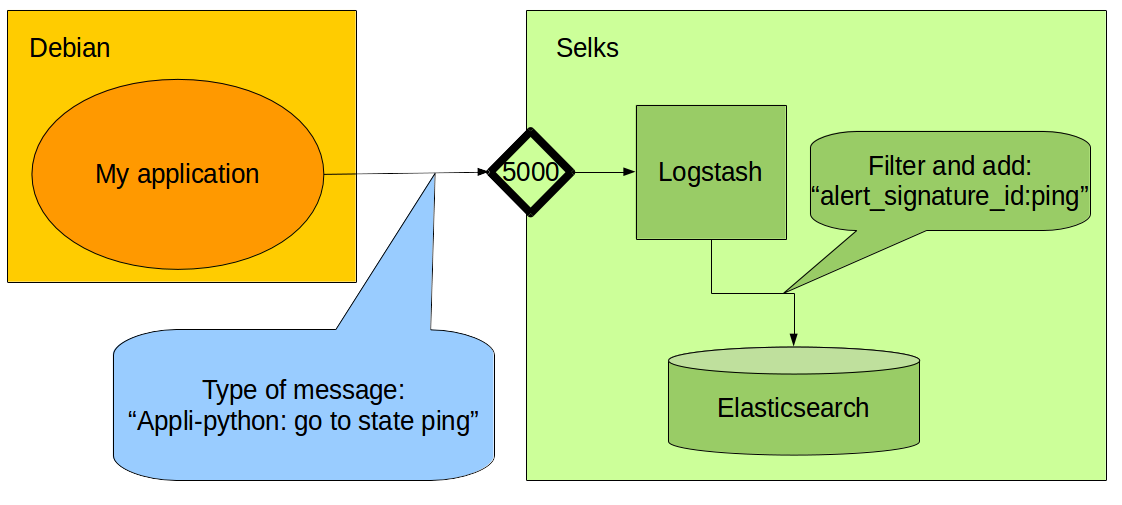
\includegraphics[width=\textwidth]{traitement_donnes}
  \caption{Data processing}
  \label{fig:dataprocessing}
\end{figure}


\section{SIEM}
\label{sec:SIEM}

I also achieve to implement a SIEM. To do so, I used the <<elasticsearch>> library for python. With it I can make
request to the data base easily. I collect the last events, I refresh the interface with these information, and
analyze its. After analysis, I am able to say if the application is under attack.

The figure \ref{fig:mysiem} represent the interface of the SIEM implemented.


\begin{figure}[h]
  \centering
  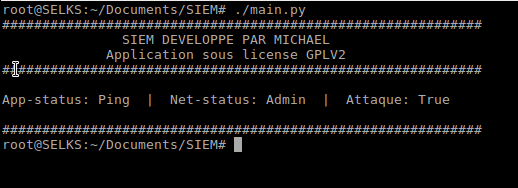
\includegraphics[width=0.7\textwidth]{siem_interface}
  \caption{My siem interface}
  \label{fig:mysiem}
\end{figure}

\newpage
\section{Summary}

The next figure represents a summary of the infrastructure of our system.

\begin{figure}[h]
  \centering
  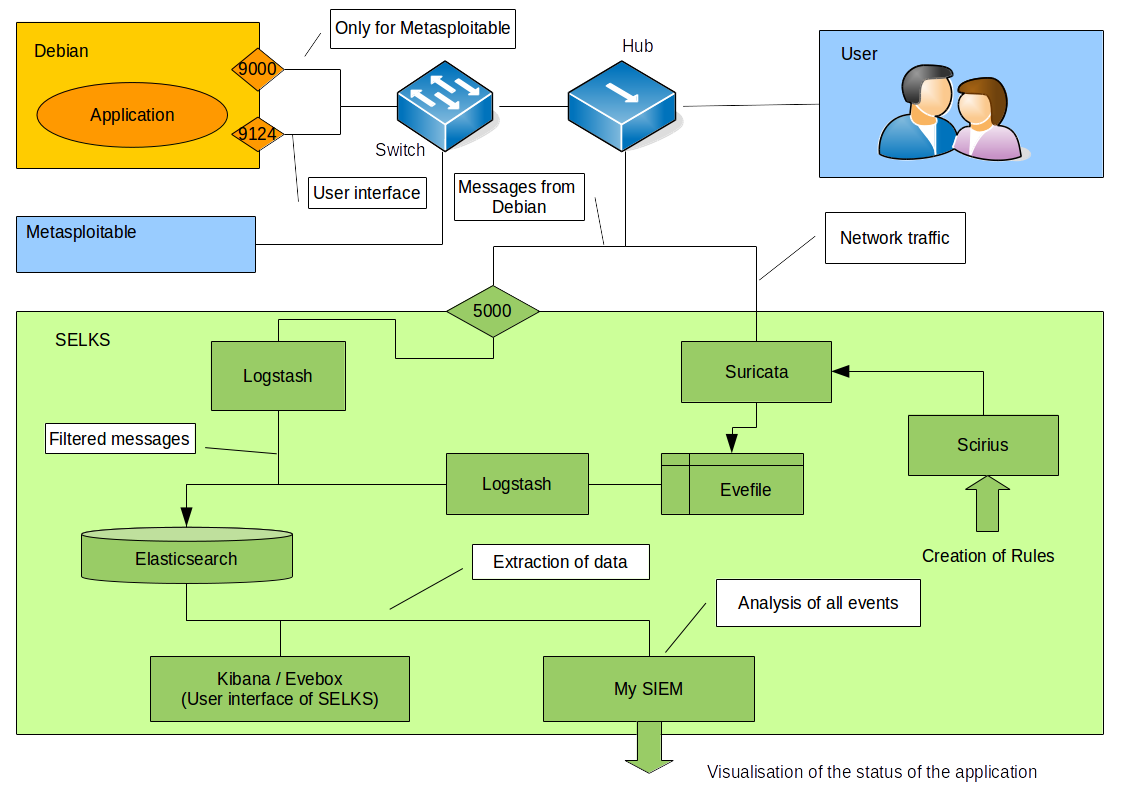
\includegraphics[width=\textwidth]{summary}
  \caption{Summary of the situation}
  \label{fig:summ}
\end{figure}

%%% Local Variables:
%%% mode: latex
%%% TeX-master: "../rapport_de_base"
%%% End:
